\documentclass[oneside,senior]{BYUIPhys}
% The BYUPhys class is for producing theses and dissertations
% in the BYU Department of Physics and Astronomy.  You can supply
% the following optional arguments in the square brackets to
% specify the thesis type:
%
%   senior  : Produces the senior thesis preliminary pages (default)
%   honors  : Produces the honors thesis preliminary pages
%   masters : Produces the masters thesis preliminary pages
%   phd     : Produces the PhD dissertation preliminary pages
%
% The default format is appropriate for printing, with blank pages
% inserted after the preliminary pages in twoside mode so you can
% send it directly to a two-sided printer. However, for ETD
% submission the blank pages need to be removed from the final output.
% The following option does this for you:
%
%   etd     : Produces a copy with no blank pages in the preliminary section.
%             Remove this option to produce a version with blank pages inserted
%             for easy double sided printing.
%
% The rest of the class options are the same as the regular book class.
% A few to remember:
%
%   oneside : Produces single sided print layout (recommended for theses less than 50 pages)
%   twoside : Produces single sided print layout (the default if you remove oneside)
%
% The BYUPhys class provides the following macros:
%
%   \makepreliminarypages : Makes the preliminary pages
%   \clearemptydoublepage : same as \cleardoublepage but doesn't put page numbers
%                           on blank intervening pages
%   \singlespace          : switch to single spaced lines
%   \doublespace          : switch to double spaced lines
%
% --------------------------- Load Packages ---------------------------------

% The graphicx package allows the inclusion of figures.  Plain LaTeX and
% pdfLaTeX handle graphics differently. The following code checks which one
% you are compiling with, and switches the graphicx package options accordingly.
\usepackage{ifpdf}
\ifpdf
\usepackage[pdftex]{graphicx}
\else
\usepackage[dvips]{graphicx}
\fi

% The fancyhdr package allows you to easily customize the page header.
% The settings below produce a nice, well separated header.
\usepackage{fancyhdr}
\fancyhead{}
\fancyhead[LO]{\slshape \rightmark}
\fancyhead[RO,LE]{\textbf{\thepage}}
\fancyhead[RE]{\slshape \leftmark}
\fancyfoot{}
\pagestyle{fancy}
\renewcommand{\chaptermark}[1]{\markboth{\chaptername \ \thechapter \ \ #1}{}}
\renewcommand{\sectionmark}[1]{\markright{\thesection \ \ #1}}

% The caption package allows us to change the formatting of figure captions.
% The commands here change to the suggested caption format: single spaced and a bold tag
\usepackage[margin=0.3in,labelfont=bf,labelsep=none]{caption}
\DeclareCaptionFormat{suggested}{\singlespace#1#2 #3\par\doublespace}
\captionsetup{format=suggested}

% The cite package cleans up the way citations are handled.  For example, it
% changes the citation [1,2,3,6,7,8,9,10,11] into [1-3,6-11].  If your advisor
% wants superscript citations, use the overcite package instead of the cite package.
\usepackage[noadjust]{cite}

% The makeidx package makes your index for you.  To make an index entry,
% go to the place in the book that should be referenced and type
%  \index{key}
% An index entry labeled "key" (or whatever you type) will then
% be included and point to the correct page.
\usepackage{makeidx}
\makeindex

% The url package allows for the nice typesetting of URLs.  Since URLs are often
% long with no spaces, they mess up line wrapping.  The command \url{http://www.physics.byu.edu}
% allows LaTeX to break the url across lines at appropriate places: e.g. http://www.
% physics.byu.edu.  This is helpful if you reference web pages.
\usepackage{url}
\urlstyle{rm}

% If you have a lot of equations, you might be interested in the amstex package.
% It defines a number of environments and macros that are helpful for mathematics.
% We don't do much math in this example, so we haven't used amstex here.
\usepackage{amsmath}

% If you need chemistry symbols you can use \usepackage{mhchem} to make them. They are made in the following way \ce{ H2O }
\usepackage{mhchem}

% Attempt to define a new math operator
\DeclareMathOperator {\myOp}{myOp}
\DeclareMathOperator {\erfc}{erfc}

% The hyperref package provides automatic linking and bookmarking for the table
% of contents, index, equation references, and figure references.  It must be
% included for the BYU Physics class to make a properly functioning electronic
% thesis.  It should be the last package loaded if possible.
%
% To include a link in your pdf use \href{URL}{Text to be displayed}.  If your
% display text is the URL, you probably should use the \url{} command discussed
% above.
%
% To add a bookmark in the pdf you can use \pdfbookmark.  You can look up its usage
% in the hyperref package documentation
\usepackage[bookmarksnumbered,pdfpagelabels=true,plainpages=false,colorlinks=true,
linkcolor=black,citecolor=black,urlcolor=blue]{hyperref}

\usepackage{listings}
\usepackage{color}
\definecolor{mygreen}{rgb}{0,0.6,0}
\definecolor{mygray}{rgb}{0.5,0.5,0.5}
\definecolor{mymauve}{rgb}{0.58,0,0.82}

\lstset{ %
	backgroundcolor=\color{white},   % choose the background color
	basicstyle=\footnotesize,        % size of fonts used for the code
	breaklines=true,                 % automatic line breaking only at whitespace
	captionpos=b,                    % sets the caption-position to bottom
	commentstyle=\color{mygreen},    % comment style
	escapeinside={\%*}{*)},          % if you want to add LaTeX within your code
	keywordstyle=\color{blue},       % keyword style
	stringstyle=\color{mymauve},     % string literal style
}
%
% To allow centering of items in tables use the array package
\usepackage{array}  % for example 1
% and define new column types.  See the LaTeX tips chapter
\newcolumntype{P}[1]{>{\centering\arraybackslash}p{#1}} % for example 1
\newcolumntype{M}[1]{>{\centering\arraybackslash}m{#1}}  % for example 1

% ------------------------- Fill in these fields for the preliminary pages ----------------------------
%
% For Senior and honors this is the year and month that you submit the thesis
% For Masters and PhD, this is your graduation date
\Year{2021}
\Month{January}
\Author{Todd Lines}

% If you have a long title, split it between two lines. The \TitleBottom field defines the second line
% A two line title should be an "inverted pyramid" with the top line longer than the bottom.
% If you have one line use just \TitleTop. If you have just two lines use \TitleTop and \TitleMiddle
% If you have three lines use \TitleTop, \TitleMiddle, and \TitleBottom
% But try to not make your title too long.  If one or two lines can work, use that.
\TitleTop{ORBITS AS CONIC SECTIONS SHOWING THAT A DISTANCE}
\TitleMiddle{SQUARED LAW GIVES AN ELLIPTICAL ORBIT}
%  \TitleBottom{}

% Your research advisor
\Advisor{Lance Nelson}

% Your committee members beyond your advisor
\MemberA{Ryan Nielson}
\MemberB{Brian Tonks}
\ThesisCoordinator{Evan Hansen}

% The representative of the department who will approve your thesis (usually the chair)
\DepRep{R. Todd Lines}

% The title of the department representative
\DepRepTitle{Chair}


% The text of your abstract
\Abstract{The abstract is a \emph{summary} of the thesis, \emph{not an
		introduction}. Keep in mind that abstracts are often published
	separately from the paper they summarize. In your abstract, give a
	concise synopsis of the work, emphasizing the conclusions; you
	need not include the supporting arguments for the conclusions. The
	purpose of the abstract is to help prospective readers decide
	whether to read your thesis, but your goal is not necessarily to
	persuade people to read your thesis. In fact, a successful
	abstract enables people to get an accurate overall view of your
	work without needing to read it. Usually, an abstract contains a
	single paragraph, but it can have more if absolutely necessary.
	Remember to state the subject of the paper immediately followed by
	a summary of the experimental or theoretical results and the
	methods used to obtain them. Avoid equations, graphics, and
	citations; if a citation is essential it must be cited fully
	within the abstract. Keep the abstract factual. Avoid vague statements
	like, ``Conclusions are drawn," or ``the significance of the experiment
	is discussed."  State the conclusions and findings outright in the abstract.}

% Acknowledge those who helped and supported you
\Acknowledgments{
	This page is optional. You may acknowledge whom you will---your
	advisor, colleagues, family members. Please keep acknowledgments
	in good taste. I would like to acknowledge Dr. Kristine Hansen and Dr.
	Elizabeth Hedengren, whose Advanced Writing Seminar motivated this project.
	I also wish to thank Jean-Fran\c{c}ois Van Huele, Steven Turley, and Ross
	Spencer for reviewing this document and for ripping it to shreds
	as every good advisor should do to a thesis draft.
}

\fussy

\begin{document}
	
	% Start page counting in roman numerals
	\frontmatter
	
	% This command makes the formal preliminary pages.
	% You can comment it out during the drafting process if you want to save paper.
	\makepreliminarypages
	
	\singlespace
	
	% Make the table of contents.
	\tableofcontents
	\clearemptydoublepage
	
	% Make the list of figures
	\listoffigures
	\clearemptydoublepage
	
	\doublespace
	
	% Start regular page counting at page 1
	\mainmatter
	
	%\include{Chapter1}
	%\include{Chapter2}
	%\include{Chapter3}
	
	\chapter{Orbits}
In the following sections, we show that orbits are really conic sections. The case of a circular orbit is just a special case.
\section{Eliptical orbits}


\begin{figure}[H]
	\begin{center}
	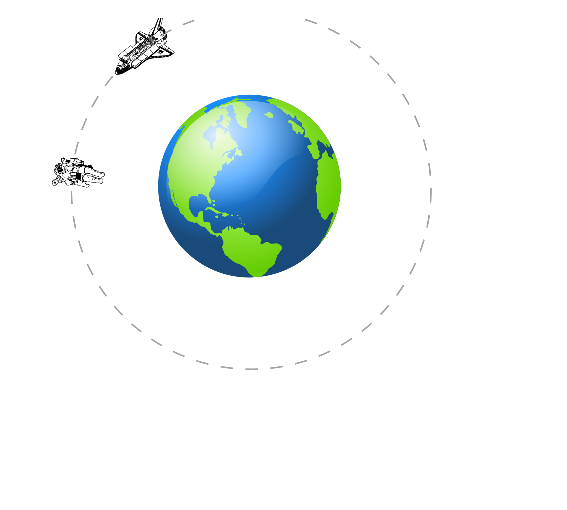
\includegraphics[width=0.3\textwidth]{orbit_figure}	
	\caption{A PH121 Circular Orbit, It's not Enough!}
\end{center}
\end{figure}


\begin{figure}[h!]
	\begin{center}
		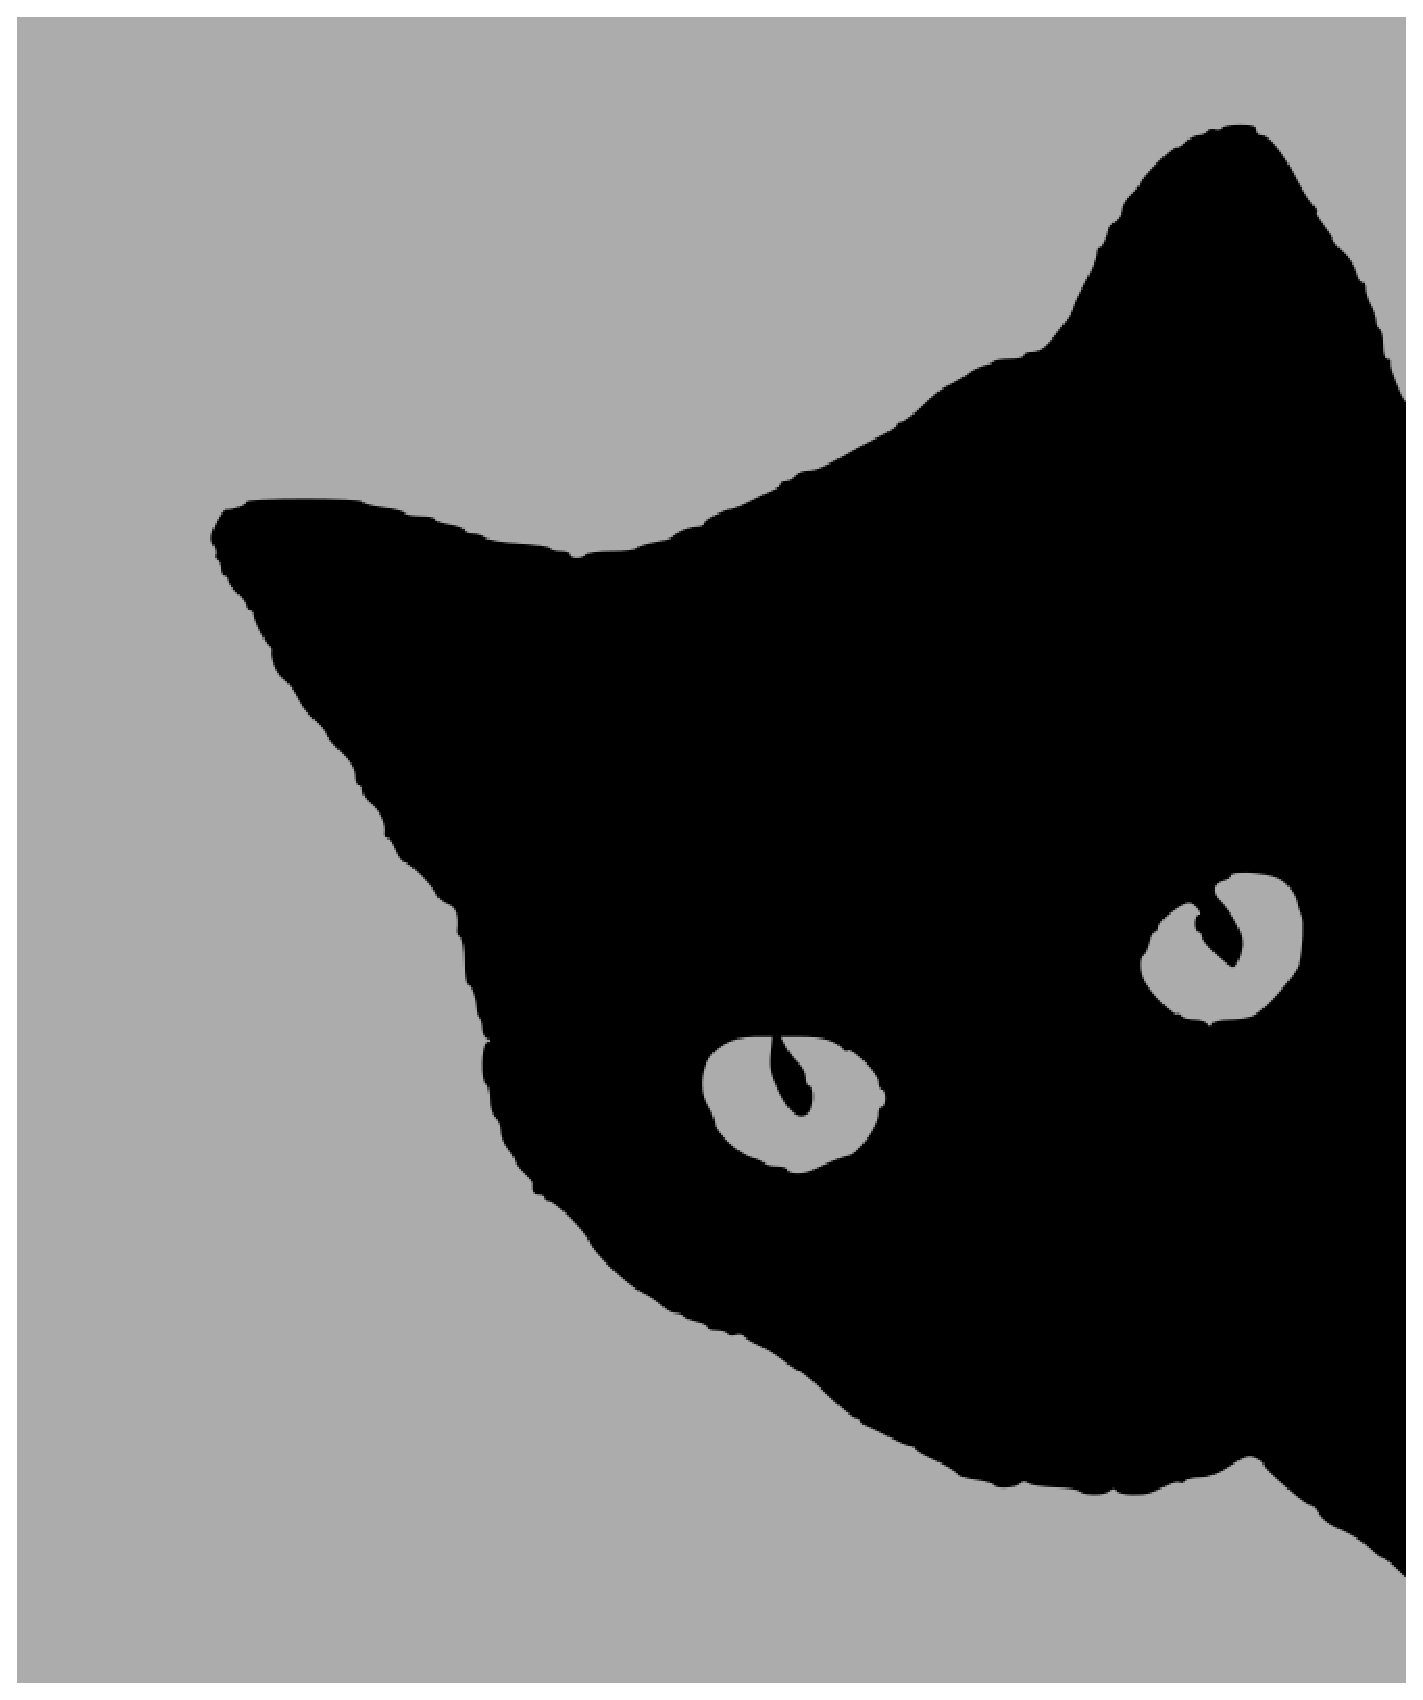
\includegraphics[width=0.4\textwidth]{cat}	
		\caption{A mistake}
	\end{center}
\end{figure}

In all our work in PH121 we used circular orbits. Kepler said orbits

should be elliptical. And that is true. We won't go though this in class,

but showing that Newton's law of gravitation implies an ellipse is a great

way to show off our new mathematics of dot and cross products. So if you are

comfortable with our new math, and curious to see how orbits work, read on.


Let's start with Newton's second law for our orbiting satellite again.

\begin{align*}
\overrightarrow{W}&=-m_{s}\overrightarrow{a}\\
&=-m_{s}g\left( r\right) \hat{r}\\
&=-m_{s}\left( G\frac{M_{E}}{r_{Es}^{2}}\right) \hat{r}
\end{align*}




We can write this as 

$$
-m_{s}\overrightarrow{a}-m_{s}\left( G\frac{M_{E}}{r_{Es}^{2}}\right) \hat{r}=0
$$


The subscripts may become burdensome, so we will drop them now, but remember

that $r=r_{Es}$ is the distance from the satellite to the Earth center of

mass to center of mass. 

$$-m_{s}\overrightarrow{a}-m_{s}\left( G\frac{M_{E}}{r^{2}}\right) \hat{r}=0$$

In the next section we will find that conservation of energy is important \ref{ConservationEnergy}. Notice that I used a marker to come up with the section number automatically.

\section{Conservation of Orbital Mechanical Energy\label{ConservationEnergy}}


Now we are going to do something strange. For no apparent reason, lets

compute the dot product of both sides of this equation 

$$\overrightarrow{v}\cdot \left( m_{s}\overrightarrow{a}+m_{s}\left( G\frac{M_{E}}{r^{2}}\right) \hat{r}\right) =\overrightarrow{v}\cdot 0 $$

then 

$$\overrightarrow{v}\cdot m_{s}\overrightarrow{a}+\overrightarrow{v}\cdot m_{s}\left( G\frac{M_{E}}{r^{2}}\right) \hat{r}=0 $$

or

$$m_{s}\overrightarrow{v}\cdot \overrightarrow{a}+m_{s}\left( G\frac{M_{E}}{r^{2}}\right) \overrightarrow{v}\cdot \hat{r}=0 $$

Now we need to learn a little bit more about dot products mixed with

derivatives. We have a position vector $\overrightarrow{r}=r\hat{r}$ The

derivative of this position vector is 

$$\frac{d\overrightarrow{r}}{dt}=\frac{d}{dt}\left( r\hat{r}\right) $$

$$=r\frac{d\hat{r}}{dt}+\frac{dr}{dt}\hat{r}$$


so if we take 

$$\frac{d\overrightarrow{r}}{dt}\cdot \hat{r}=\left( r\frac{d\hat{r}}{dt}+\frac{dr}{dt}\hat{r}\right) \cdot \hat{r}$$


$$=r\frac{d\hat{r}}{dt}\cdot \hat{r}+\frac{dr}{dt}\hat{r}\cdot \hat{r}$$%

$$=0+\frac{dr}{dt}$$%

since $d\hat{r}/dt=0.$


So 

$$\frac{d\overrightarrow{r}}{dt}\cdot \hat{r}=\frac{dr}{dt}$$

and we recognize 

\begin{equation*}
	\overrightarrow{v}=\frac{d\overrightarrow{r}}{dt}
\end{equation*}%
so we can write 
\begin{equation}
	\overrightarrow{v}\cdot \hat{r}=\frac{dr}{dt}  \label{vdotrhat}
\end{equation}%
and we have this in our orbit equation. Our orbit equation becomes

\begin{equation*}
	m_{s}\overrightarrow{v}\cdot \overrightarrow{a}+m_{s}\left( G\frac{M_{E}}{%
		r_{Es}^{2}}\right) \frac{d\overrightarrow{r}}{dt}\cdot \hat{r}=0
\end{equation*}%
or just

\begin{equation*}
	m_{s}\overrightarrow{v}\cdot \overrightarrow{a}+m_{s}\left( G\frac{M_{E}}{%
		r^{2}}\right) \frac{dr}{dt}=0
\end{equation*}

We can do something similar for the first term We can recognize 

$$\overrightarrow{a}=\frac{d\overrightarrow{v}}{dt}$$

and that $\overrightarrow{v}=v\hat{v}$ where $\hat{v}$ is a unit vector in

the same direction $\overrightarrow{v}.$ Then 

$$\frac{d\overrightarrow{v}}{dt}=\frac{d}{dt}\left( v\hat{v}\right) $$

$$=v\frac{d\hat{v}}{dt}+\frac{dv}{dt}\hat{v}$$

and 

$$\overrightarrow{v}\cdot \overrightarrow{a}=\overrightarrow{v}\cdot \frac{d\overrightarrow{v}}{dt}$$

$$=\overrightarrow{v}\cdot \left( v\frac{d\hat{v}}{dt}+\frac{dv}{dt}\hat{v}\right)
$$

$$=v\hat{v}\cdot v\frac{d\hat{v}}{dt}+v\hat{v}\cdot \frac{dv}{dt}\hat{v}$$

$$=0+v\frac{dv}{dt}\hat{v}\cdot \hat{v}$$

$$=v\frac{dv}{dt}$$

so our orbit equation becomes

$$m_{s}v\frac{dv}{dt}+m_{s}\left( G\frac{M_{E}}{r_{Es}^{2}}\right) \frac{dr}{dt}=0
$$
Now let's play a clever mathematical trick. Let's take the derivative of the
kinetic energy with respect to time.

$$\frac{d}{dt}\left( \frac{1}{2}mv^{2}\right) =\frac{1}{2}m\frac{d}{dt}\left(v^{2}\right) 
$$%
$$=\frac{1}{2}m\left( 2v\frac{dv}{dt}\right) 
$$%
$$=mv\frac{dv}{dt}$$%
Notice that this is in our orbit equation! So then%

$$m_{s}v\frac{dv}{dt}+m_{s}\left( G\frac{M_{E}}{r^{2}}\right) \frac{dr}{dt}=0
$$%
becomes 

$$\frac{d}{dt}\left( \frac{1}{2}mv^{2}\right) +m_{s}\left( G\frac{M_{E}}{r^{2}}\right) \frac{dr}{dt}=0$$%
We can play this trick again for the second term%

$$
\frac{d}{dt}\left( G\frac{M_{E}}{r}\right) =GM_{E}\frac{d}{dt}\left( \frac{1}{r}\right) 
$$
	
$$
=GM_{E}\left( -\frac{1}{r^{2}}\frac{dr}{dt}\right) 
$$
which once again we recognize this as part of our orbit equation so we can

write 

$$\frac{d}{dt}\left( \frac{1}{2}mv^{2}\right) -m_{s}\frac{d}{dt}\left( G\frac{M_{E}}{r}\right) =0$$

or 

$$\frac{d}{dt}\left( \left( \frac{1}{2}mv^{2}\right) -m_{s}\left( G\frac{M_{E}}{r}\right) \right) =0 
$$%
which tells us that 

$$
\left( \frac{1}{2}mv^{2}\right) -m_{s}\left( G\frac{M_{E}}{r_{Es}}\right) =\text{constant} 
$$
That is, the mechanical energy is conserved since we recognize this as just 
$$K+U_{g}=\text{constant} $$

And this makes sense. There are no energy loss mechanisms in our orbit. Our

masses are particles (no tidal forces inside the objects, etc.) So we expect

conservation of energy in forming our orbit.


\section{Conservation of Orbital Angular Momentum}


Now, let's do just what we did before only let's use a cross product with 
$\overrightarrow{r}$. 

$$\overrightarrow{r}\times \left( -m_{s}\overrightarrow{a}-m_{s}\left( G\frac{M_{E}}{r^{2}}\right) \hat{r}\right) =\overrightarrow{r}\times 0
$$

$$-\overrightarrow{r}\times m_{s}\overrightarrow{a}-\overrightarrow{r}\times m_{s}\left( G\frac{M_{E}}{r^{2}}\right) \hat{r}=0
$$

$$m_{s}\overrightarrow{r}\times \overrightarrow{a}+m_{s}G\frac{M_{E}}{r^{2}}\overrightarrow{r}\times \hat{r}=0
$$

$$m_{s}\overrightarrow{r}\times \overrightarrow{a}+m_{s}G\frac{M_{E}}{r^{2}}r\hat{r}\times \hat{r}=0
$$

The last term has $\hat{r}\times \hat{r}.$ The angle between $\hat{r}$ and $\hat{r}$ must be zero (they are in the same direction) so 
$$\hat{r}\times \hat{r}=\left( 1\right) \left( 1\right) \sin \left( 0\right) =0$$

and we are left with 

$$m_{s}\overrightarrow{r}\times \overrightarrow{a}=0$$

which really does note seem to helpful, but it is. Consider that 

$$\overrightarrow{a}=\frac{d^{2}\overrightarrow{r}}{dt^{2}}$$

so 

$$\overrightarrow{r}\times \overrightarrow{a}=\overrightarrow{r}\times \frac{d^{2}\overrightarrow{r}}{dt^{2}}$$

$$=\overrightarrow{r}\times \frac{d^{2}\left( r\hat{r}\right) }{dt^{2}}$$


Now consider the quantity 

$$\frac{d}{dt}\left( \overrightarrow{r}\times \frac{d\overrightarrow{r}}{dt}\right)=\overrightarrow{r}\times\frac{d^{2}\overrightarrow{r}}{dt^{2}}+\frac{d\overrightarrow{r}}{dt}\times \frac{d\overrightarrow{r}}{dt}$$

The second term must be zero because the angle between any vector and itself

must be zero and $\sin \left( 0\right) =0$, but the first term is just what

we have in our equation! so our equation becomes%

$$m_{s}\overrightarrow{r}\times \overrightarrow{a}=m_{s}\frac{d}{dt}\left( \overrightarrow{r}\times \frac{d\overrightarrow{r}}{dt}\right) =0$$

which we can write as%

$$\frac{d}{dt}\left( \overrightarrow{r}\times m_{s}\frac{d\overrightarrow{r}}{dt}\right) =0$$

$$\frac{d}{dt}\left( \overrightarrow{r}\times m_{s}\overrightarrow{v}\right) $$



$$=\frac{d}{dt}\left( \overrightarrow{L}\right) =0$$

and, hurray! we have conservation of angular momentum for our general orbit!


\section{Conic Section Equation}
You may not be a thrilled as I\ was at this point, but what we have done is typical for physicists. We use the power of mathematics and some ingenuity to predict what motions will be. You might say, \textquotedblleft but I\  would never think of taking cross and dot products seemingly randomly to find a result.\textquotedblright\ This may be true now, but as you get used to using the mathematical tools an operation like this may become more obvious. In any case, recall that early physicists spent many years trying out ways to use their mathematical tools. So eventually someone was bound to try our cross and dot product tricks. But we have only shown conservation of energy and angular momentum. We have not reached our goal. So let's return to our basic motion equation that we started with 
\begin{equation*}
	-m_{s}\overrightarrow{a}-m_{s}\left( G\frac{M_{E}}{r^{2}}\right) \hat{r}=0 
\end{equation*}
and now let's consider our equation for angular momentum
\begin{equation*}
	\overrightarrow{L}=\overrightarrow{r}\times m_{s}\overrightarrow{v}
\end{equation*}
and form the cross product of the first equation with $\overrightarrow{L}$
\begin{equation*}
	\left( -m_{s}\overrightarrow{a}-m_{s}\left( G\frac{M_{E}}{r^{2}}\right) \hat{%
		r}\right) \times \overrightarrow{L}=0\times \overrightarrow{L}
\end{equation*}
\begin{equation*}
	m_{s}\overrightarrow{a}\times \overrightarrow{L}+m_{s}\left( G\frac{M_{E}}{%
		r^{2}}\right) \hat{r}\times \overrightarrow{L}=0 
\end{equation*}
Again this may not seem like an obvious thing to do! But we find that
\begin{equation*}
	m_{s}\overrightarrow{a}\times \overrightarrow{L}=-\left( G\frac{M_{E}}{r^{2}}%
	\right) \hat{r}\times \overrightarrow{L}
\end{equation*}
and it is time for another mathematical trick. Consider the quantity
\begin{equation*}
	\frac{d}{dt}\left( \overrightarrow{v}\times \overrightarrow{L}\right) =%
	\overrightarrow{v}\times \frac{d\overrightarrow{L}}{dt}+\frac{d%
		\overrightarrow{v}}{dt}\times \overrightarrow{L}
\end{equation*}
\begin{equation*}
	=\overrightarrow{v}\times \frac{d}{dt}\left( \overrightarrow{r}\times m_{s}%
	\overrightarrow{v}\right) +\overrightarrow{a}\times \overrightarrow{L}
\end{equation*}
\begin{equation*}
	=\overrightarrow{v}\times \left( 0\right) +\overrightarrow{a}\times 
	\overrightarrow{L}
\end{equation*}
\begin{equation*}
	=\overrightarrow{a}\times \overrightarrow{L}
\end{equation*}
for our situation because we have already shown that angular momentum is
conserved. So we have
\begin{equation*}
	m_{s}\frac{d}{dt}\left( \overrightarrow{v}\times \overrightarrow{L}%
	\right)=-\left( G\frac{M_{E}}{r^{2}}\right) \hat{r}\times \overrightarrow{L}
\end{equation*}
Now let's look at the right hand side. Writing out the angular momentum gives
\begin{equation*}
	\hat{r}\times \overrightarrow{L}=\hat{r}\times \left( \overrightarrow{r}%
	\times m_{s}\overrightarrow{v}\right) 
\end{equation*}
and I will use a vector product identity that I\ will let the math department teach you
\begin{equation*}
	\overrightarrow{A}\times \left( \overrightarrow{B}\times \overrightarrow{C}%
	\right) =\overrightarrow{B}\left( \overrightarrow{A}\cdot \overrightarrow{C}%
	\right) -\overrightarrow{C}\left( \overrightarrow{A}\cdot \overrightarrow{B}%
	\right) 
\end{equation*}%
so for us
\begin{equation*}
	\overrightarrow{r}\times \overrightarrow{L}=m_{s}\hat{r}\times \left( 
	\overrightarrow{r}\times \overrightarrow{v}\right) 
\end{equation*}%
\begin{equation*}
	=m_{s}\left( \overrightarrow{r}\left( \hat{r}\cdot \overrightarrow{v}\right)
	-\overrightarrow{v}\left( \hat{r}\cdot \overrightarrow{r}\right) \right) 
\end{equation*}%
\begin{equation*}
	=m_{s}\left( \overrightarrow{r}\left( \hat{r}\cdot \overrightarrow{v}\right)
	-\overrightarrow{v}r\right) 
\end{equation*}%
We already know from equation (\ref{vdotrhat}) that%
\begin{equation*}
	\overrightarrow{v}\cdot \hat{r}=\frac{dr}{dt}
\end{equation*}%
then 
$$\hat{r}\times \overrightarrow{L}=m_{s}\left( r\hat{r}\left( \frac{dr}{dt}\right) -\overrightarrow{v}r\right) $$
then finally 
$$ m_{s}\frac{d}{dt}\left( \overrightarrow{v}\times \overrightarrow{L}\right)=-\left( G\frac{M_{E}m_{s}}{r^{2}}\right) \left( r\hat{r}\left( \frac{dr}{dt}\right) -\overrightarrow{v}r\right) 
$$
$$=-\left( GM_{E}m_{s}\right) \left[ \left( \frac{dr}{dt}\right) \frac{\hat{r}}{r}-\frac{\overrightarrow{v}}{r}\right] $$
Let's employ one more mathematical trick
$$\frac{d}{dt}\left( \frac{\overrightarrow{r}}{r}\right) =-\overrightarrow{r} \frac{1}{r^{2}}\frac{dr}{dt}+\frac{1}{r}\frac{d\overrightarrow{r}}{dt}
$$
$$=-\overrightarrow{r}\frac{1}{r^{2}}\frac{dr}{dt}+\frac{1}{r}\overrightarrow{v}
$$
$$=-\left( \hat{r}\frac{1}{r}\frac{dr}{dt}-\frac{1}{r}\overrightarrow{v}\right)$$
and this is the part of our equation that I\ wrote in square brackets, so with a substitution our equation becomes
$$m_{s}\frac{d}{dt}\left( \overrightarrow{v}\times \overrightarrow{L}\right)=\left( GM_{E}m_{s}\right) \left( \frac{d}{dt}\left( \frac{\overrightarrow{r}}{r}\right) \right) $$
or, canceling the $dt$ factors from both sides
$$m_{s}d\left( \overrightarrow{v}\times \overrightarrow{L}\right) =\left(GM_{E}m_{s}\right) \left( d\left( \frac{\overrightarrow{r}}{r}\right)\right)
$$
and we can integrate both sides
$$m_{s}\int d\left( \overrightarrow{v}\times \overrightarrow{L}\right)=-\left( GM_{E}m_{s}\right) \int \left( d\left( \frac{\overrightarrow{r}}{r}\right) \right)
$$
to find 
$$m_{s}\overrightarrow{v}\times \overrightarrow{L}=\left( GM_{E}m_{s}\right)\left( \frac{\overrightarrow{r}}{r}\right) +\overrightarrow{B}
$$
where $\overrightarrow{B}$ is a vector constant of integration. Once again for no apparent reason let's take the dot product of this equation with $\overrightarrow{r}$
$$\overrightarrow{r}\cdot \left( m_{s}\overrightarrow{v}\times \overrightarrow{L}\right) =-\left( GM_{E}m_{s}\right) \overrightarrow{r}\cdot \left( \frac{\overrightarrow{r}}{r}\right) +\overrightarrow{r}\cdot \overrightarrow{B} 
$$
and use another vector product identity
$$\overrightarrow{A}\cdot \overrightarrow{B}\times \overrightarrow{C}=\overrightarrow{A}\times \overrightarrow{B}\cdot \overrightarrow{C} 
$$
We can write this as to write our dot product equation as 
$$\left( m_{s}\overrightarrow{r}\times \overrightarrow{v}\right) \cdot \overrightarrow{L}=\left( GM_{E}m_{s}\right) r+rB\cos \theta _{rB} 
$$
or
$$\frac{1}{m_{s}}\left( \overrightarrow{r}\times m_{s}\overrightarrow{v}\right) \cdot \overrightarrow{L}=\left( GM_{E}m_{s}\right) r+rB\cos \theta_{rB}
$$
$$\left( \overrightarrow{r}\times m_{s}\overrightarrow{v}\right) \cdot \overrightarrow{L}=\left( GM_{E}m_{s}\right) r+rB\cos \theta _{rB} 
$$
$$\overrightarrow{L}\cdot \overrightarrow{L}=\left( GM_{E}m_{s}\right)r+rB\cos \theta _{rB} 
$$
$$L^{2}=\left( GM_{E}m_{s}\right) r+rB\cos \theta _{rB} 
$$
and now we can solve for $r$
$$L^{2}=r\left( \left( GM_{E}m_{s}\right) +B\cos \theta _{rB}\right) 
$$
then 

$$r=\frac{L^{2}}{\left( \left( GM_{E}m_{s}\right) +B\cos \theta _{rB}\right) } 
$$
or, rearranging slightly, 
$$r=\frac{L^{2}/\left( GM_{E}m_{s}\right) }{\left( 1+\left(B/GM_{E}m_{s}\right) \cos \theta _{rB}\right) } $$
If we compare this to the parametric equation for a conic section (straight out of your calculus text book), 
$$r=\frac{p}{1+e\cos \nu } $$
we can see that our orbit must be a conic section with a semi-latus rectum, 
$$p=L^{2}/\left( GM_{E}m_{s}\right) $$
and an eccentricity, 
$$e=B/GM_{E}m_{s}$$
and an angle 
$$\nu =\theta _{rB}$$
This means our orbit could be any conic section, circle, ellipse, parabola, or hyperbola. For satellites we most often choose ellipses. But the other conic sections are possible.So Kepler was partially right. An ellipse is a general form for an orbit, but it might even be better to write Kepler's law to say that orbits are conic sections.

If you are a normal PH121 student, your reaction to this problem might be \textquotedblleft Agh, maybe I should change my major to horticulture!\textquotedblright\ But don't worry, This was really a junior level problem, and for us physics majors we have many classes (both physics and math classes) to take before we would be expected to do a problem like this. Still it is fun to see that we \emph{can} do a problem like this with the math we learned in lowly PH121 if we are very persistent!  Interested students can read more in the the book \textit{Fundamentals of Astrodynamics} by Bate \textit{et. al.} \cite{Bate1971}\cite{ExplainingComputers2021}\cite{byuiphysics}\cite{Acquista76}
	

	\chapter{Numerical Verification of the Orbit Equation}
Let's start with a long meaningless quotation so we can see how quotations are done.

\begin{quotation}
Four score and seven years ago our fathers brought forth on this continent, a new nation, conceived in Liberty, and dedicated to the proposition that all men are created equal.

Now we are engaged in a great civil war, testing whether that nation, or any nation so conceived and so dedicated, can long endure. We are met on a great battle-field of that war. We have come to dedicate a portion of that field, as a final resting place for those who here gave their lives that that nation might live. It is altogether fitting and proper that we should do this.

But, in a larger sense, we can not dedicate -- we can not consecrate -- we can not hallow -- this ground. The brave men, living and dead, who struggled here, have consecrated it, far above our poor power to add or detract. The world will little note, nor long remember what we say here, but it can never forget what they did here. It is for us the living, rather, to be dedicated here to the unfinished work which they who fought here have thus far so nobly advanced. It is rather for us to be here dedicated to the great task remaining before us -- that from these honored dead we take increased devotion to that cause for which they gave the last full measure of devotion -- that we here highly resolve that these dead shall not have died in vain -- that this nation, under God, shall have a new birth of freedom -- and that government of the people, by the people, for the people, shall not perish from the earth.
\end{quotation}
Now some text outside the quotation. There is very little \ce{ O2 } in space.  
\section[Long Section Names]{Some section names are way to long to appear in the table of contents so you need to include a short title for the TOC}
This is an example of a section name that is too long.  You should shorten it if you can, but if you can't this long name will mess up the Table of Contents.  So there is an option to include a short title.  Put the short section nave version in square brackets before the actual (long) section name (in curly brackets).


	\chapter{Long Quotations}
Let's start with a long meaningless quotation so we can see how quotations are done.

\begin{quotation}
	Four score and seven years ago our fathers brought forth on this continent, a new nation, conceived in Liberty, and dedicated to the proposition that all men are created equal.
	
	Now we are engaged in a great civil war, testing whether that nation, or any nation so conceived and so dedicated, can long endure. We are met on a great battle-field of that war. We have come to dedicate a portion of that field, as a final resting place for those who here gave their lives that that nation might live. It is altogether fitting and proper that we should do this.
	
	But, in a larger sense, we can not dedicate -- we can not consecrate -- we can not hallow -- this ground. The brave men, living and dead, who struggled here, have consecrated it, far above our poor power to add or detract. The world will little note, nor long remember what we say here, but it can never forget what they did here. It is for us the living, rather, to be dedicated here to the unfinished work which they who fought here have thus far so nobly advanced. It is rather for us to be here dedicated to the great task remaining before us -- that from these honored dead we take increased devotion to that cause for which they gave the last full measure of devotion -- that we here highly resolve that these dead shall not have died in vain -- that this nation, under God, shall have a new birth of freedom -- and that government of the people, by the people, for the people, shall not perish from the earth.
\end{quotation} 
Now some text outside the quotation.
\section{Chemical Equations in \LaTeX}
If you need chemistry symbols you can use
\verb|\usepackage{mhchem}| which must be in the preamble of your main document.
They are made in the following way \verb|\ce{ H2O }| becomes \ce{ H2O }.
There is very little \ce{ O2 } in space.  
\section[Long Section Names]{Some section names are way to long to appear in the table of contents so you need to include a short title for the TOC}
This is an example of a section name that is too long.  You should shorten it if you can, but if you can't this long name will mess up the Table of Contents.  So there is an option to include a short title.  Put the short section nave version in square brackets before the actual (long) section name (in curly brackets).
Here is a random numbered list.
\begin{enumerate}
	\item one item that is long so we can see the hanging indent happen and because a hanging indent looks better, don't you think so?
	\item a second item, $2 \pi$
	
\end{enumerate}

\section{Double figures}
Sometimes it is useful to have two figures side by side. One way to do this is with a minipage environment. Here is an example of doing just that. Notice that I had to adjust the caption sizes to make the figures line up nicely. I used a \verb|\vspace| command to adjust the vertical spacing of the second figure. There are probably more elegant ways of doing this.

\begin{figure}[htb!]
	\centering
	\begin{minipage}{.45\textwidth}
		\centering
		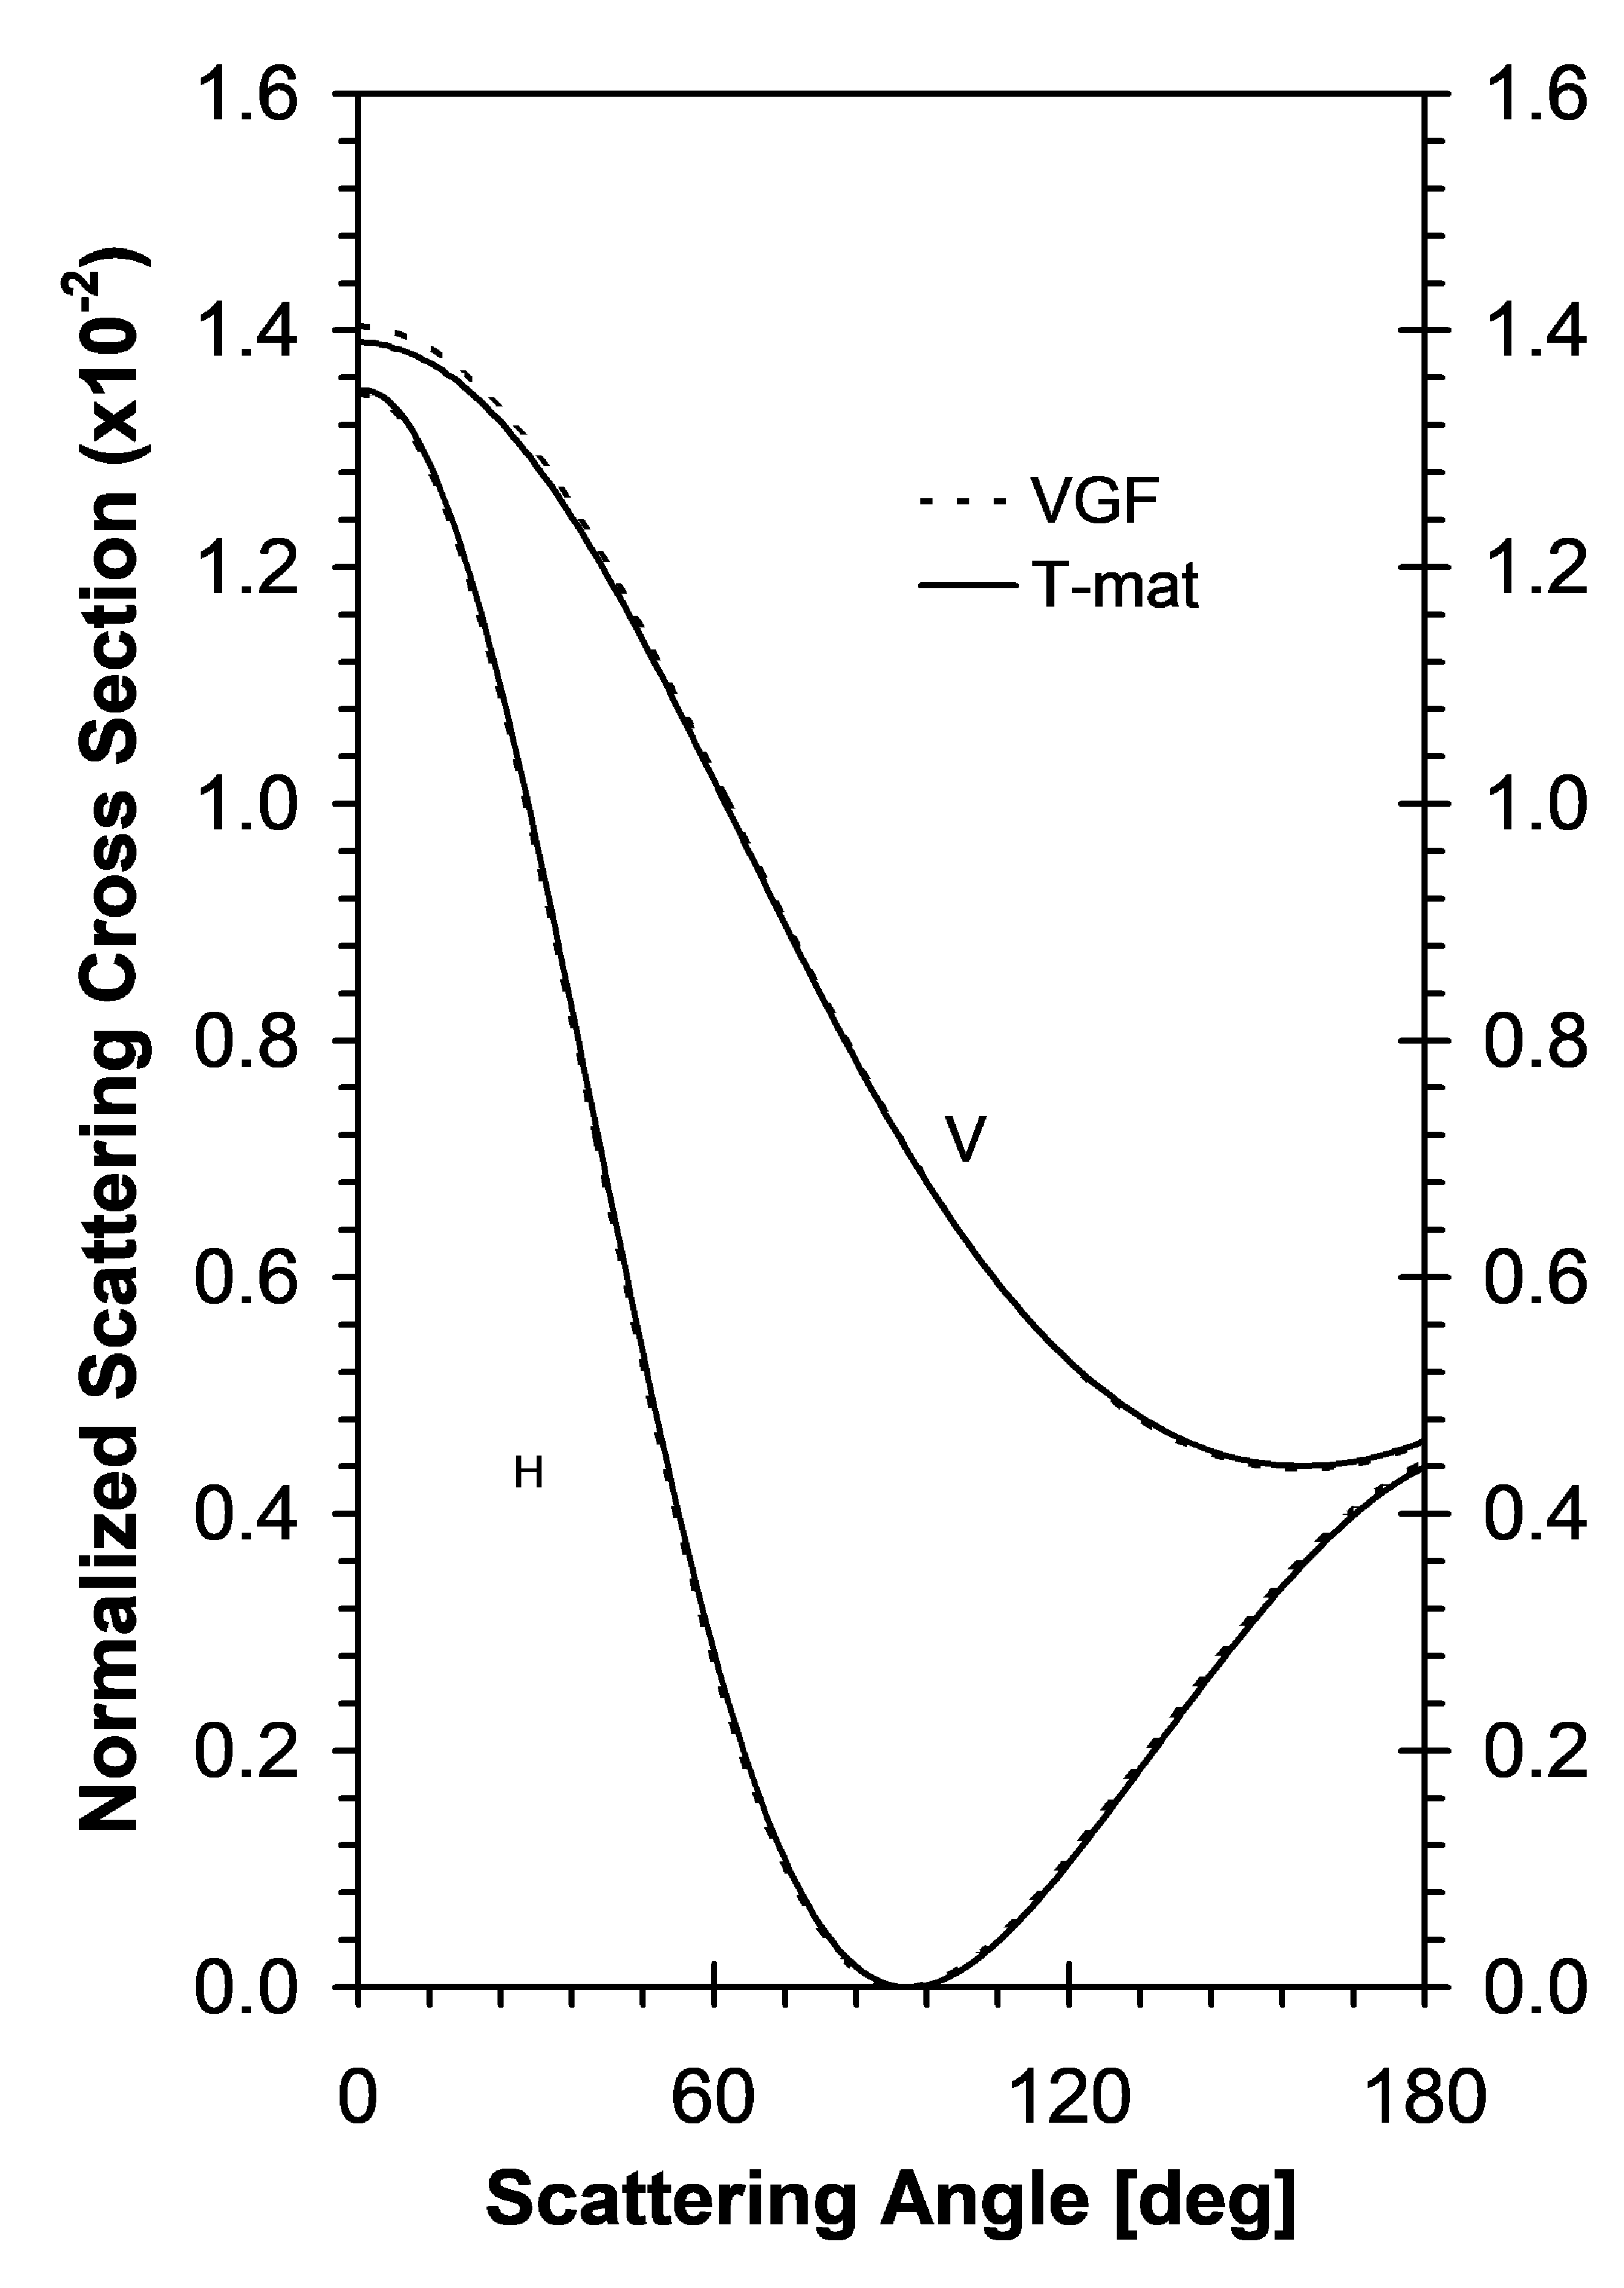
\includegraphics[width=0.8\linewidth, height=0.35\textheight]{test60b}
		\caption[short caption A]{A longer caption A}
	    \label{fig:bigsphere1}
	\end{minipage} \hfill
	\begin{minipage}{0.45\textwidth}
		\centering
		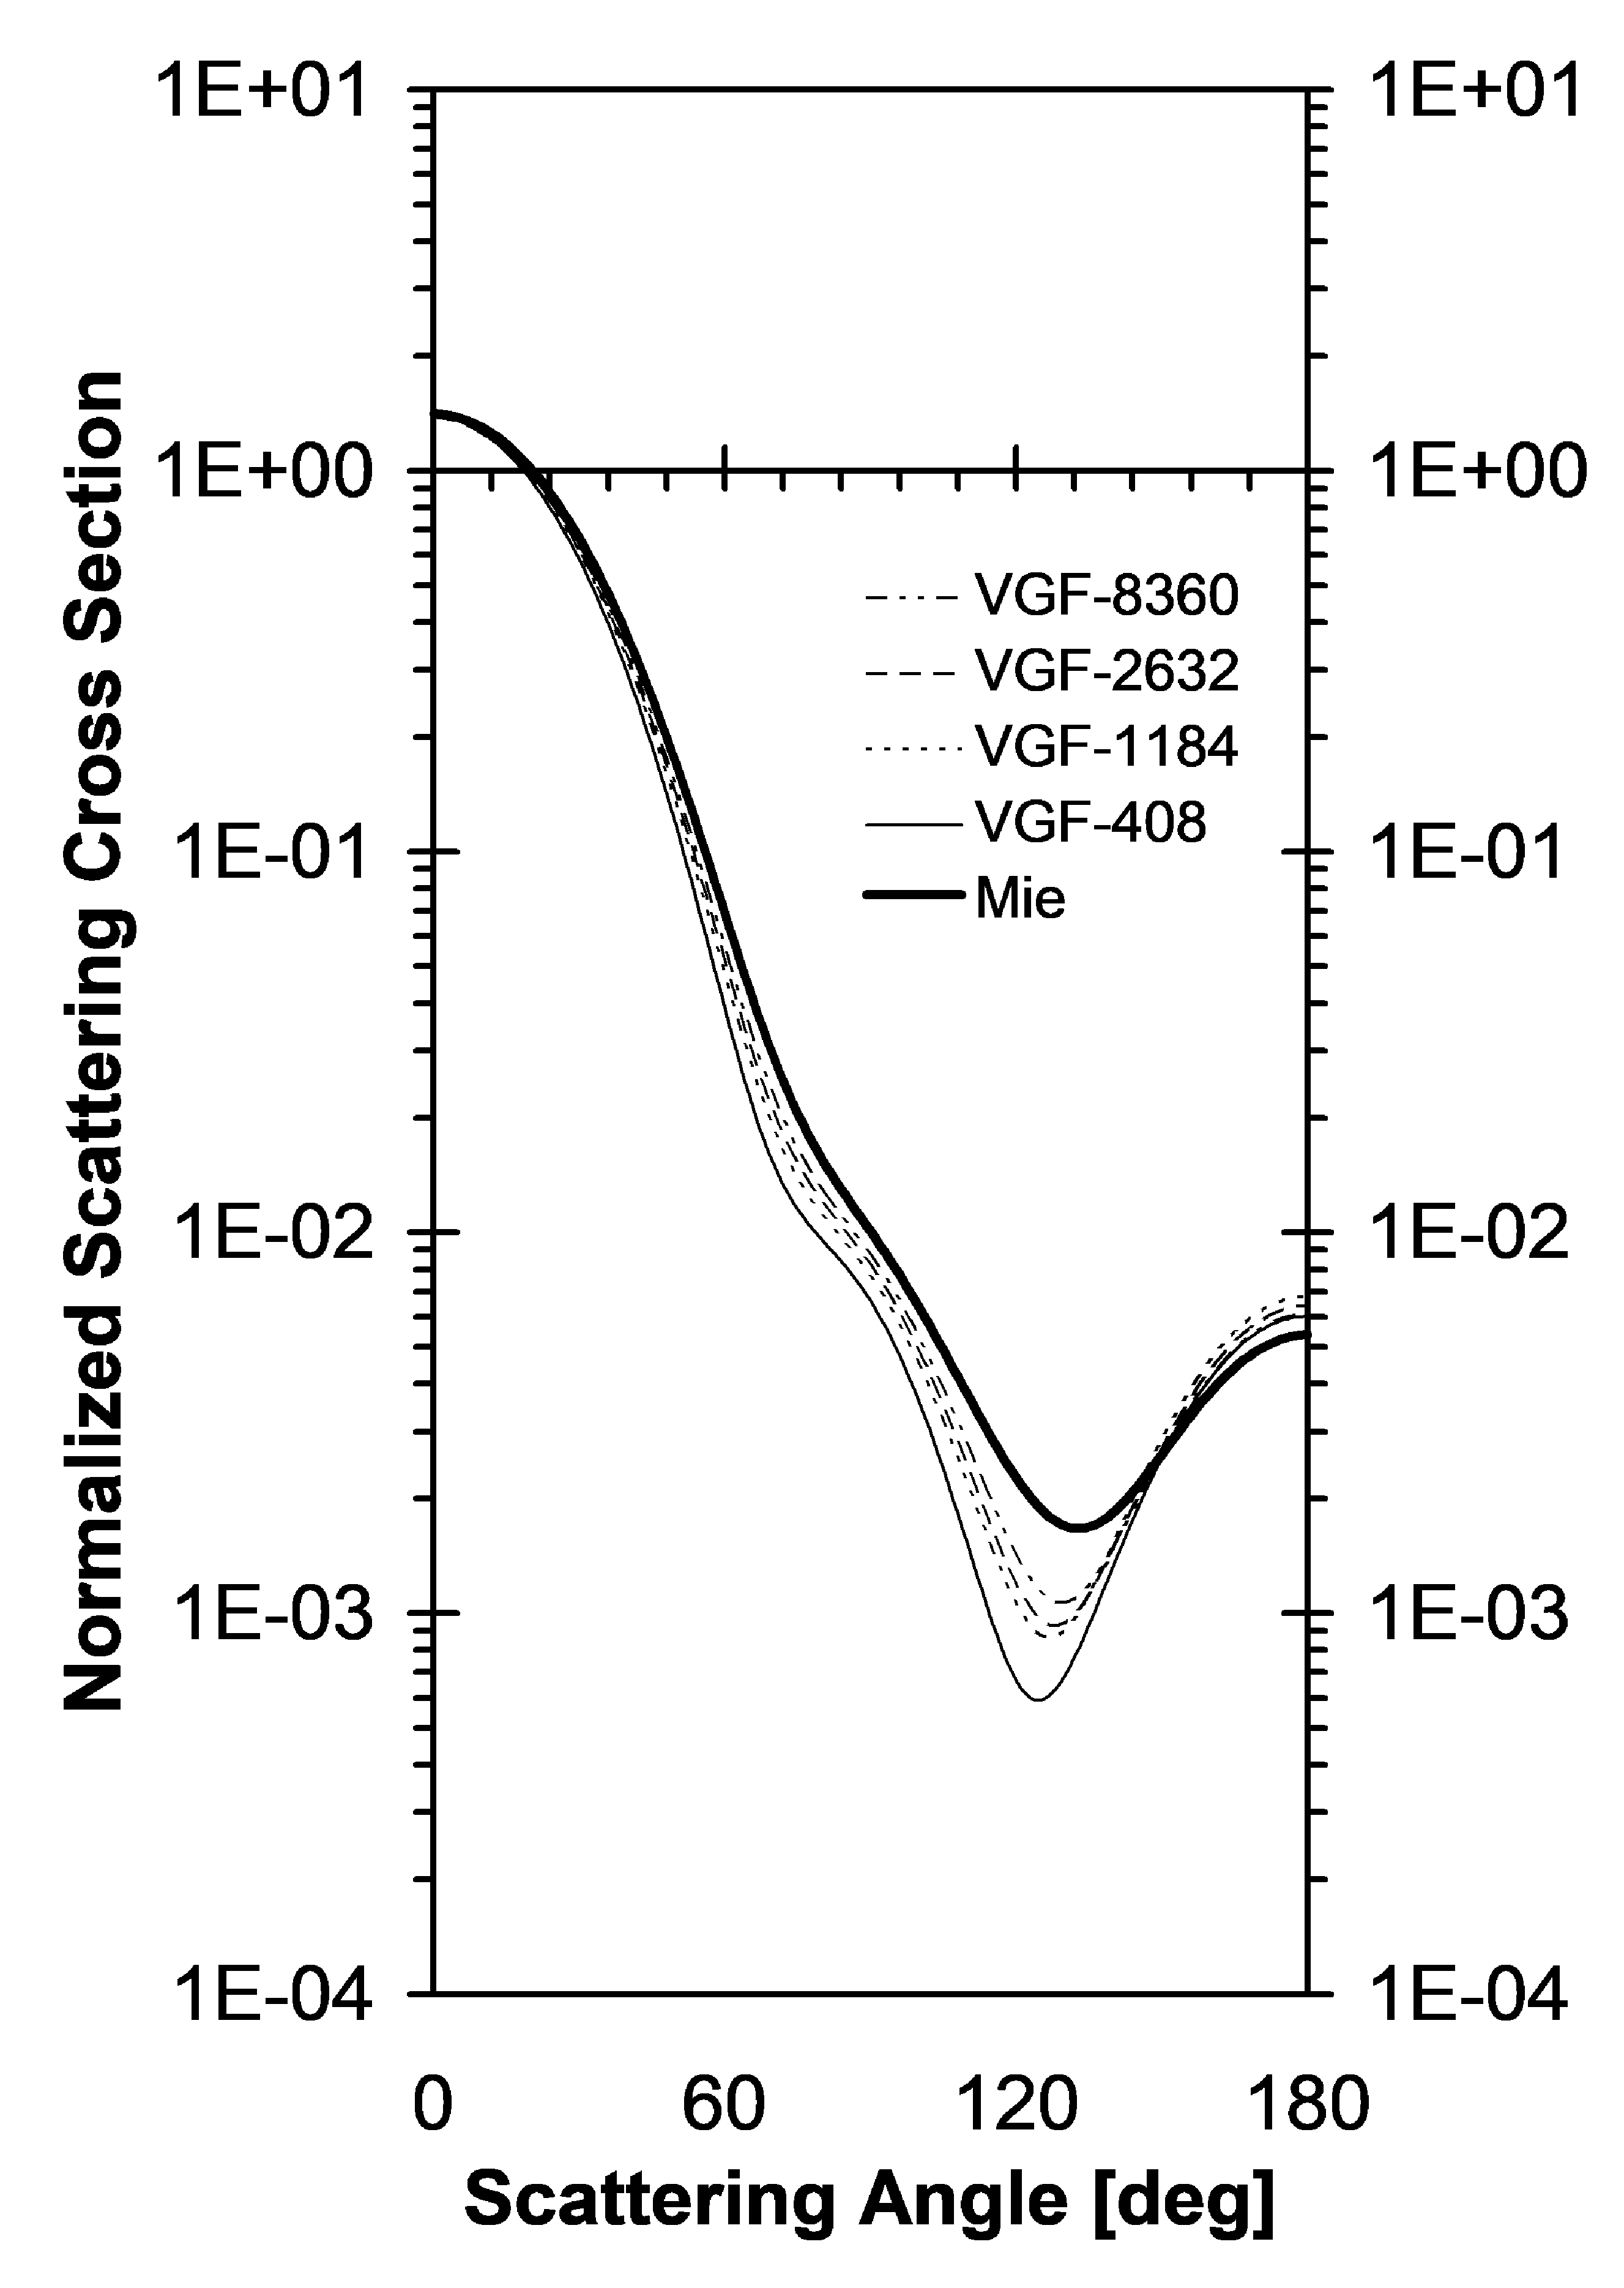
\includegraphics[width=0.9\linewidth, height=0.35\textheight]{test70}
		\caption{Caption b goes here}
		\label{fig:bigsphere2}
	\end{minipage}
\end{figure}
You might want to have different figures all as part of a larger figure. I recommend making the graphics as all one piece.  For example see figure \ref{fig:bigsphere1} and \ref{fig:bigsphere2}.
\section{defining new math operators}
This can be done with the following commands
\begin {verbatim}
   \DeclareMathOperator {\myOp}{myOp}
   \myOp(x)
\end{verbatim}
The first line needs to be in the preamble of your document. The second is put into math where you want the new operator to apperar. Then when you use the new operator it looks like this
$$\myOp(x)$$
Let's try this with erfc for the error function. Then we want to add 
\begin {verbatim}
\DeclareMathOperator {\erfc}{erfc}
\end{verbatim}
to the preamble and 
\begin {verbatim}
\erfc(x)
\end{verbatim} 
to the text where we want it.  It should look like this
$$\erfc(x)$$
or in the text $\erfc(x)$.
You might also want to put normal text in an equation. Like 
$$ \frac{x^2+distance^2}{r^2}$$
Note that the word ``distance'' doesn't look right. Using the 
\begin {verbatim}
   \textrm{normal text}
\end{verbatim}
command fixes this.
$$ \frac{x^2+\textrm{distance}^2 }{r^2}$$.
\section{Tables}
There is a lot to \LaTeX tables. I have more to write on this. But centering can be a difficulty.  Here are examples of doing that.

Example 1
Use the array package and define a new column type with horizontal or vertical centering (or both).  

\begin{verbatim}
	\newcolumntype{M}[1]{>{\centering\arraybackslash}m{#1}}
\end{verbatim} line above. Then in the column definitions in your table replace  the ``p'' with an ``M.'' 
\begin{table}[h]
	\centering
	\begin{tabular}[c]{|M{2.5cm}|M{1.5cm}|M{1.5cm}|M{1.5cm}|M{1.5cm}|M{1.5cm}|M{1.5cm}|} \hline
		Samples & \multicolumn{2}{|c|}{Data Item 1} & \multicolumn{2}{|c|}{Data Item 2} & \multicolumn{2}{|c|}{Data Item 3}\\ \hline
		Lifetime ($\tau$)     & 1     & 2     & 1     & 2     & 1     & 2     \\ \hline
		Average Lifetime (ps) & 116.5 & 464.2 & 114.7 & 404.7 & 115.3 & 414.7 \\ \hline
		Intensity (\%)        & 69    & 31    & 64.5  & 35.5  & 66.2  & 33.8  \\ \hline
	\end{tabular}
	\caption{This is the table caption}
	\label{OpenResults}
\end{table}

Example 2:
I use this one a lot.  Just put \textbackslash hfil  in each cell you want centered.

\begin{table}[h]
	\centering
	\begin{tabular}[c]{|p{2.5cm}|p{1.5cm}|p{1.5cm}|p{1.5cm}|p{1.5cm}|p{1.5cm}|p{1.5cm}|} \hline
			Samples & \multicolumn{2}{|c|}{Data Item 1} & \multicolumn{2}{|c|}{Data Item 2} & \multicolumn{2}{|c|}{Data Item 3}\\ \hline
		Lifetime ($\tau$)     & \hfil 1     & \hfil 2     & \hfil 1     & \hfil 2     & \hfil 1     & \hfil 2 \\  \hline
		Average Lifetime (ps) & \hfil 116.5 & \hfil 464.2 & \hfil 114.7 & \hfil 404.7 & \hfil 115.3 & \hfil 414.7 \\ \hline
		Intensity (\%)        & \hfil 69    & \hfil 31    & \hfil 64.5  & \hfil 35.5  & \hfil 66.2  & \hfil 33.8 \\ \hline
	\end{tabular}
	\caption{This is the table caption}
	\label{OpenResults}
\end{table}

Example 3:
The last example was a trick.  Maybe a ``better'' way to go is to put \textbackslash centering in the cells you want centered.

\begin{table}[h]
	\centering
	\begin{tabular}[c]{|p{2.5cm}|p{1.5cm}|p{1.5cm}|p{1.5cm}|p{1.5cm}|p{1.5cm}|p{1.5cm}|} \hline
		Samples & \multicolumn{2}{|c|}{Data Item 1} & \multicolumn{2}{|c|}{Data Item 2} & \multicolumn{2}{|c|}{Data Item 3}\\ \hline
		Lifetime ($\tau$)      & 1     & 2     & 1     & 2     & 1     & 2     \\  \hline
		Average Lifetime (ps)  & 116.5 & 464.2 & 114.7 & 404.7 & 115.3 & 414.7 \\  \hline
		Intensity (\%)         & 69    & 31    & 64.5  & 35.5  & 66.2  & 33.8  \\  \hline
	\end{tabular}
	\caption{This is the table caption}
	\label{OpenResults}
\end{table}



	
	
	\appendix
	
	
	\bibliographystyle{phBYU}
	\bibliography{orbits}
	
	\chapter{Things that belong in an appendix} 
\label{app:BelongInApp}

The purpose of an appendix is to provide supplementary information
which would distract if included in the main body of the thesis.
Items appearing as an appendix might include lengthy derivations. If
students feel compelled to include a brief tutorial on relevant
background information (not new research), it should appear as an
appendix. An appendix might consist of portions of unique computer
code that was developed as part of the project.  
	\chapter{Including Your Code} \label{AppendixCode}
\label{app:Talk}

You might want to include some code in your thesis. This is done with a lstlisting environment. Using lstlisting provides syntax highlighting. 

\begin{lstlisting}[language=Python] 
x=10
y=x**2
print('Helo world', y)
\end{lstlisting}

A whole code might look like this

\small
\begin{lstlisting}[language=Python]
#############################################################
# Program to do a curve fit in python with a user defined 
#  fit equation and %  with data supplied by the user.
# The user types the data into numpy arrays by hand,
#  and supplies a function with the fit equation.
#  In this example, the function is called RC_Charging.
#
# Author:  Todd Lines
# Date:    2023-02-20
#############################################################
import numpy as np
import matplotlib.pyplot as plt
from scipy.optimize import curve_fit

# Define the Gaussian function
print("  ")
print("Find a curve fit to a user defined function")

#Here is where you define the function to use in the fit
def RC_Charging(x, A, B):
x=np.longdouble(x)
y = A*(1-np.exp(-B*x))
return y

#here is where you give the data to fit. Put it into numpyu arrays
xdata = np.array([10,    20,   30,   40,  50,   60,   70,   80,   
90,  100, 110, 120,  130,  140,  150,  160,  
170,  180])
ydata = np.array([0.5, 0.76, 0.97, 1.15, 1.3, 1.42, 1.54, 1.64, 
1.73, 1.82, 1.9, 1.97,2.05, 2.12, 2.18, 2.24, 
2.28, 2.33])

#Now plot the data so we can see the data points
plt.plot(xdata, ydata, 'o')


#Now perform the curve fit. We can't just use a linear fit. 
#  The data is very much #  not linear. So we will use a more 
#  robust curve fit rotine from scipy. The sciepy optimize 
#  curve_fit() routine needs the equation to use for the
#  fit as a function (here RC_Charting()) and it needs the 
#  fit parameters and for the error on 
#  the fit parameters we need the covariance matrix to be output
parameters, covariance = curve_fit(RC_Charging, xdata, ydata)

#Pull out the fit prameters
fit_A = parameters[0]
fit_B = parameters[1]


#Pull out the uncertanty from the diagonal elements of the 
#  covariance matrix. Remember that the diagonal elements 
#  are the error squared.
SE = np.sqrt(np.diag(covariance))
SE_A = SE[0]
SE_B = SE[1]

#Use the fit parameters to make a set of estamated y values 
#  from the fit equation. We can pass in the whole xdata array
#  and get out all the y value estimates at once using our 
#  function with our fit equation.  I called the new y-values
#  fit_y.
fit_y = RC_Charging(xdata, fit_A, fit_B)

#Plot the data (as dots) and the fit (as a line) to see if the equation
#  makes sense as a good fit.
plt.xlabel('Time in seconds')
plt.ylabel('Voltage (V)')
plt.plot(xdata, ydata, 'ro', label='data')
plt.plot(xdata, fit_y, 'b-', label='fit')
plt.legend()

#and print out our fit parameters and their uncertainties
print("  ")
print(F'The value of A is {fit_A:.5f} with standard error of {SE_A:.5f}.')
print(F'The value of B is {fit_B:.5f} with standard error of {SE_B:.5f}.')
print("  ")

#sometimes the curve fit routine throws a math warning, let the user know 
#  that the program ended and not to be upset about the warning
print("successful end of program, warning about overflow may follow")
print("  ")
\end{lstlisting}
\normalsize
It can do other languages, like the C language.

\small
\begin{lstlisting}[language=C] 
#include "ran0.h"
float ran0(int* idum)
{
	static float y,maxran,v[98];
	float dum;
	static int iff=0;
	int j;
	unsigned i,k;
	
	if((*idum < 0)||(iff == 0))
	{
		iff=1;
		i=2;
		maxran = RAND_MAX+1.0;
		*idum=1;
		for(j=1;j<97;j++)
		{
			dum=rand();
		}
		for(j=1;j<=97;j++)
		{
			v[j]=rand();
		}
		y=rand();
	}
	j=1+97.0*y/maxran;
	if((j>97)||(j<1))
	{
		cout << "This cannot happen." << endl;
		exit(0);
	}
	y = v[j];
	v[j] = rand();
	return y/maxran;
};
\end{lstlisting}
\normalsize

But if you don't need syntax highlighting (like if you will print in only black and white) you can also use a verbatim environment. In both cases, \LaTeX \enspace doesn't try to interpret your computer program code as \LaTeX \enspace commands. I want to make sure the code fits on the page, so for the verbatum envirnment example I am going to reduce the font size with a small environment as well. 
\begin{small}
\begingroup
\makeatletter
\@totalleftmargin=-1cm
	\begin{verbatim}
##############################################################
# Euler code to calculate a satellite orbit                  #
##############################################################
# Todd Lines
# 2022 04 19
##############################################################
# This code will calculate the path of an orbit given a 
#  specific velocity of the object and it's direction. 
#  It would probably be be better to have the whole calcuation 
#  go in reverse. But I didn't do that on purpose since we are
#  verifying that an elipse comes from a distance squared law
#  with this code.
##############################################################
# Load Libraries
import numpy as np                 # Numerical calculation library
import matplotlib.pyplot as plt    # Data plotting libary

##############################################################
# Initial conditions and physial setup constants
R=6371E3       # Radius of Earth in m
M=5.9E24       # Mass of plannet in Kg
m=0.020        # mass of our sattelite in kilograms
G=5.11E-11     # N*m**2/kg**2 Gravitational Constant
x0=2*R         # Initial x position in m (The Earth is at x = 0)
y0=0.5*R       # Initial y position in m (The Earth is at y = 0)
v0=6000.0       # Initial satellite velocity in m/s
thetadeg=100   # Satellite launch angle in degrees

##############################################################
## Set up the time steps and number of calcualtions
deltat=1.0        # Time steps of 0.01 seconds
ti=0              # starting at t=0
tf=300000         # final time in seconds
N=int((tf-ti)/deltat)  # calcualte how many time steps are in tf-ti seconds

##############################################################
# Preliminary calculations
pi=np.arccos(-1.0)         # calculate pi to machine percision
theta=thetadeg*pi/180      # calcualte theta in radians
vx1=v0*np.cos(theta)       # calculte the x component of the initial velocity
vy1=v0*np.sin(theta)       # calculte the y component of the initial velocity

##############################################################
# define and zero arrays
t=np.zeros((N))
x=np.zeros((N))
y=np.zeros((N))
vx=np.zeros((N))
vy=np.zeros((N))


##############################################################
## make an array of times to use
t=np.linspace(0,tf,num=N);
##############################################################
# Draw The Earth
r=R                               # distance from center in m
ThetaE0=0.00                      # initial angle in degrees
delta_ThetaE=5                    # change in angle in degrees
# calculate the number of points to use in our Earth drawing
Ne= int(360/delta_ThetaE)+1       # number of points
ye=np.zeros((Ne))
xe=np.zeros((Ne))
# Draw Circle to represent the Earth
ye[0]=0        # initial y positoin
xe[0]=r
thetaE=ThetaE0
for i in range (0,Ne):
thetaE=thetaE+delta_ThetaE
xe[i]=r*np.cos(thetaE*pi/180)
ye[i]=r*np.sin(thetaE*pi/180)
plt.plot(xe, ye)

##############################################################
# now perform an Euler's Method Calculation
# now recalling that vx(i) already has a cos(theta) in it,
# we can use this to calculate the x part of the resistive
# force and likewise use vy(i) in calculating the y part of
# the resistive force. No explicit calculation of theta is
# necessary this way, and we save lots of computation time.
x=np.zeros((N))
y=np.zeros((N))
vx=np.zeros((N))
vy=np.zeros((N))

# Put the starting point in the arrays
x[0]=x0                        # initial x position
y[0]=y0                        # initial y positoin
vx[0]=vx1                      # initial x velocity
vy[0]=vy1                      # initial y velocity, what we give it

# Now calculate all the other points of the satellite path
print('working')
for i in range (0,N-1):
r=np.sqrt(x[i]**2+y[i]**2)
if x[i] != 0:
theta=np.arctan(y[i]/x[i])
else:
theta=pi/2

if y[i]>0 and x[i]<0:
theta=pi+theta
if y[i]<0 and x[i]<=0:
theta=theta+pi
if y[i]<0 and x[i]>0:
theta=2*pi+theta
if r<R:
print("hit surface")
break   #hit surface

# Calculate the velocity and acceleration terms   
fx=vx[i]
gx=-np.cos(theta) * G*M/r**2
fy=vy[i]
gy=-np.sin(theta) * G*M/r**2

# Take an Euler step
x[i+1]=x[i]+deltat*fx
y[i+1]=y[i]+deltat*fy
vx[i+1]=vx[i]+deltat*gx
vy[i+1]=vy[i]+deltat*gy   
print('done')

# Now plot our satellite path 
plt.plot(x[:i],y[:i])
plt.show()

# And that is the end of the program
	
	\end{verbatim}
\endgroup
	
\end{small}



	
	% \phantomsection \addcontentsline{toc}{chapter}{Index}
	\renewcommand{\baselinestretch}{1} \small \normalsize
	\printindex
	
	
\end{document}
Footer
© 2023 GitHub, Inc.
Footer navigation
Terms
Privacy
Securit